\documentclass[10pt,portrait]{article}
\usepackage{amssymb,amsmath,amsthm,amsfonts}
\usepackage{multicol,multirow}
\usepackage{calc}
\usepackage{ifthen}
% \usepackage[a4paper, total={6in, 8in}]{geometry}
\usepackage[a4paper, portrait, margin=0.4in]{geometry}
\usepackage[colorlinks=true,citecolor=blue,linkcolor=blue]{hyperref}
\usepackage{graphicx}
\usepackage{cases}

\makeatletter
\renewcommand{\section}{\@startsection{section}{1}{0mm}%
                                {-1ex plus -.5ex minus -.2ex}%
                                {0.5ex plus .2ex}%x
                                {\normalfont\large\bfseries}}
\renewcommand{\subsection}{\@startsection{subsection}{2}{0mm}%
                                {-1explus -.5ex minus -.2ex}%
                                {0.5ex plus .2ex}%
                                {\normalfont\normalsize\bfseries}}
\renewcommand{\subsubsection}{\@startsection{subsubsection}{3}{0mm}%
                                {-1ex plus -.5ex minus -.2ex}%
                                {1ex plus .2ex}%
                                {\normalfont\small\bfseries}}
\makeatother
\setcounter{secnumdepth}{0}





\graphicspath{ {./images/} }







\begin{document}


% \newpage
%     \begin{center}
%          \Large{\textbf{The Story of Investment Horizon}} \\
%          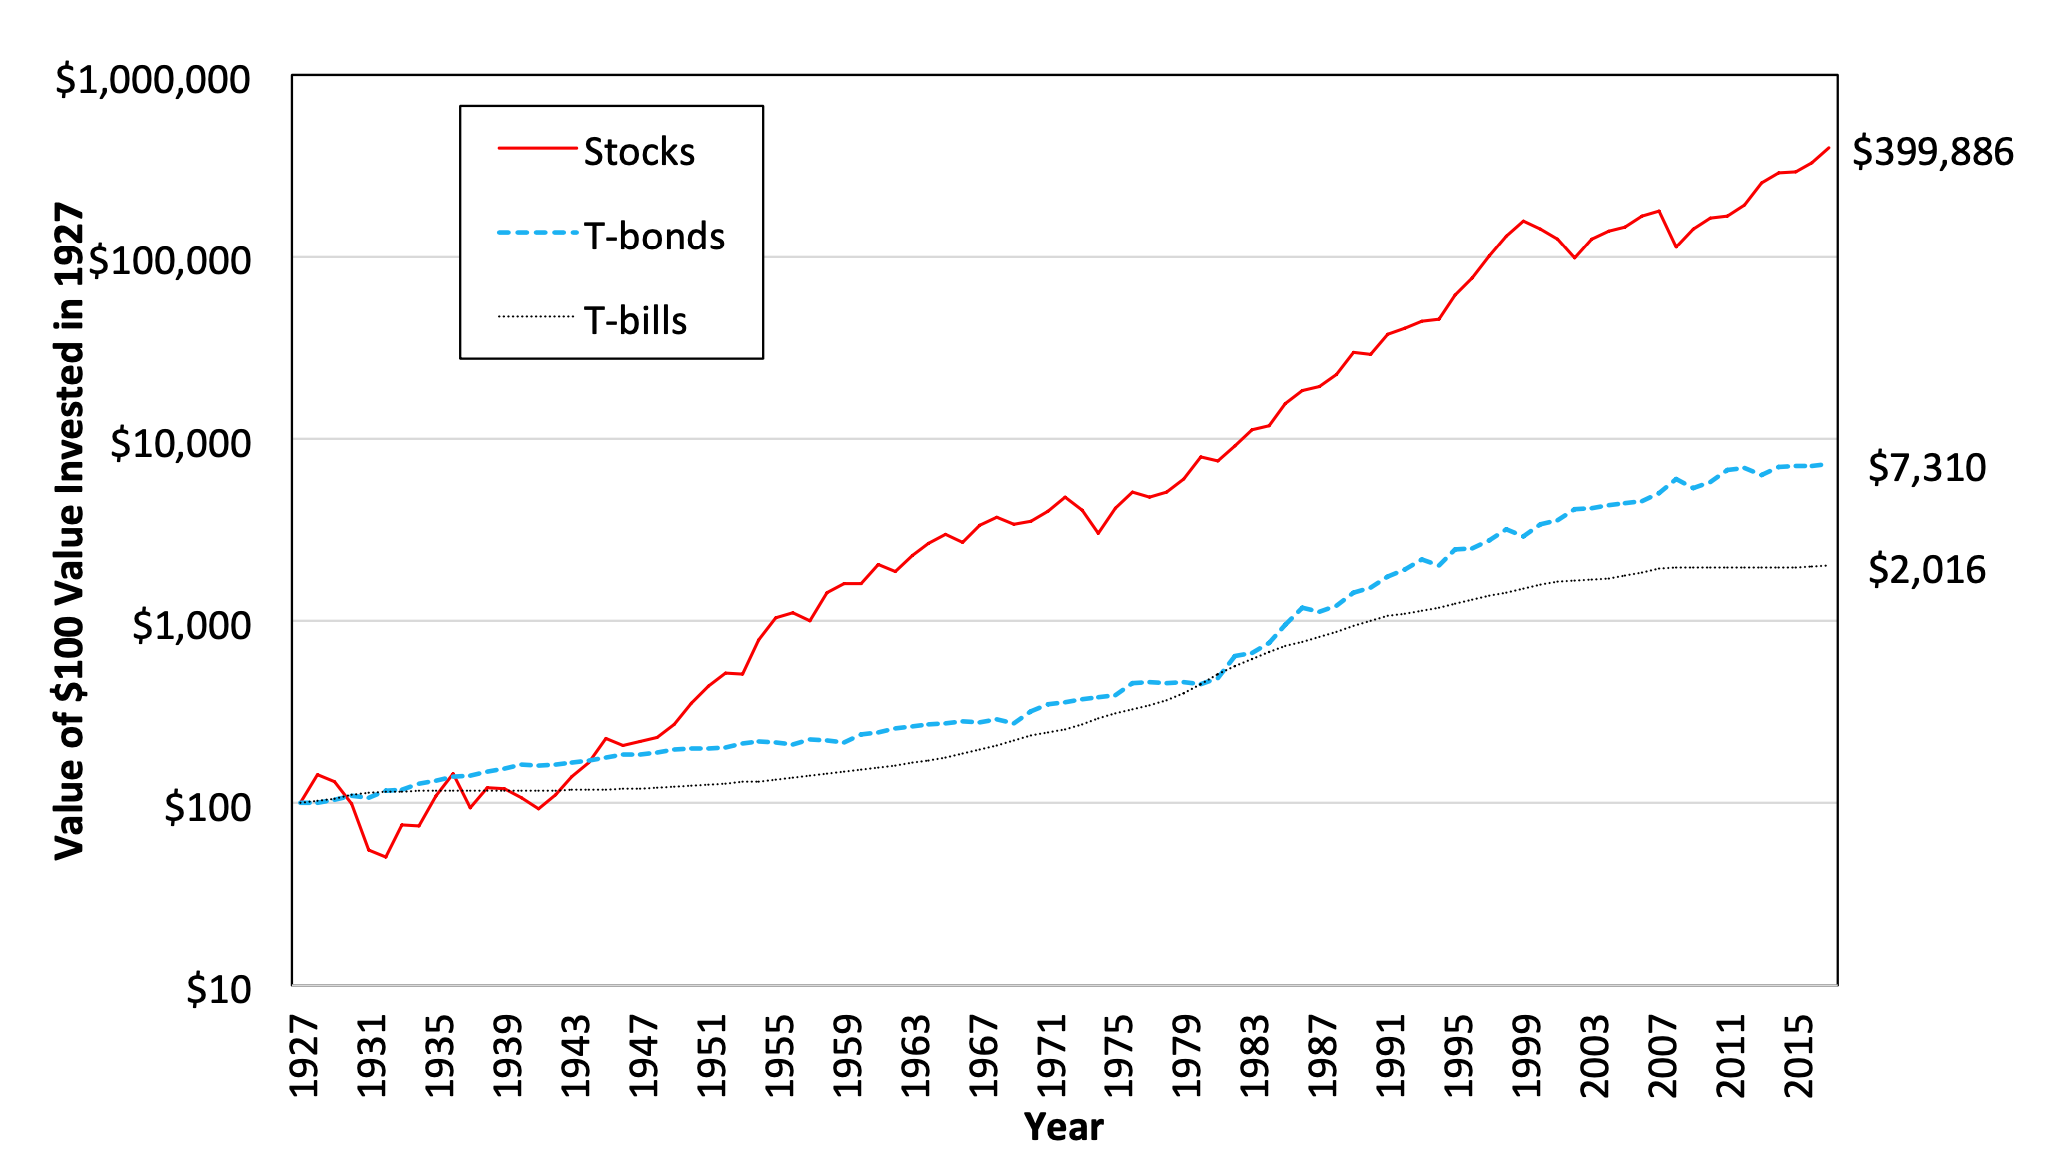
\includegraphics[width=0.8\textwidth]{asset_return_comparison}
%     \end{center}

%     \subsection{Stock is a good investment if you have long investment horizon}
%     \begin{itemize}
%         \item As we can tell from the graph, stock have significatlly greater return compared to bonds and bills.
%         \item But bear in mind that this is true when you have a long investment horizon
%         \item Put stock martket at a micro-scope level, we will experience great fluctuation everyday
%     \end{itemize}
    
%     \subsection{You can do better than stock, as long as you can take that risk}
%     \begin{itemize}
%         \item For instance, derivatives, are also a high risk asset, but the potential return is higher
%         \item During the 2008 Crisis, there is a man who lend Goldman Sachs millions of money to help the firm.
%         \item In exchange he asked for options on the stock with a low strike price
%         \item Eventually Goldman Sachs survived the crisis and the man gain billions of money
%         \item However, if we look at stock price, firms like Deutsche Bank never get out of the trouble. This trade is risky.
%     \end{itemize}

%     \subsection{Implication from my point of view}
%     \begin{itemize}
%         \item Take a long-term investment horizon and invest in things with high potential value
%         \item We need to identify firms that is with good condition that worth invest in, E.g: Goldman Sachs v.s. Deutshce Bank
%         \item This require us to know the business, how much company is involved in, the probability of it strive again.
%     \end{itemize}

%     \begin{center}
%         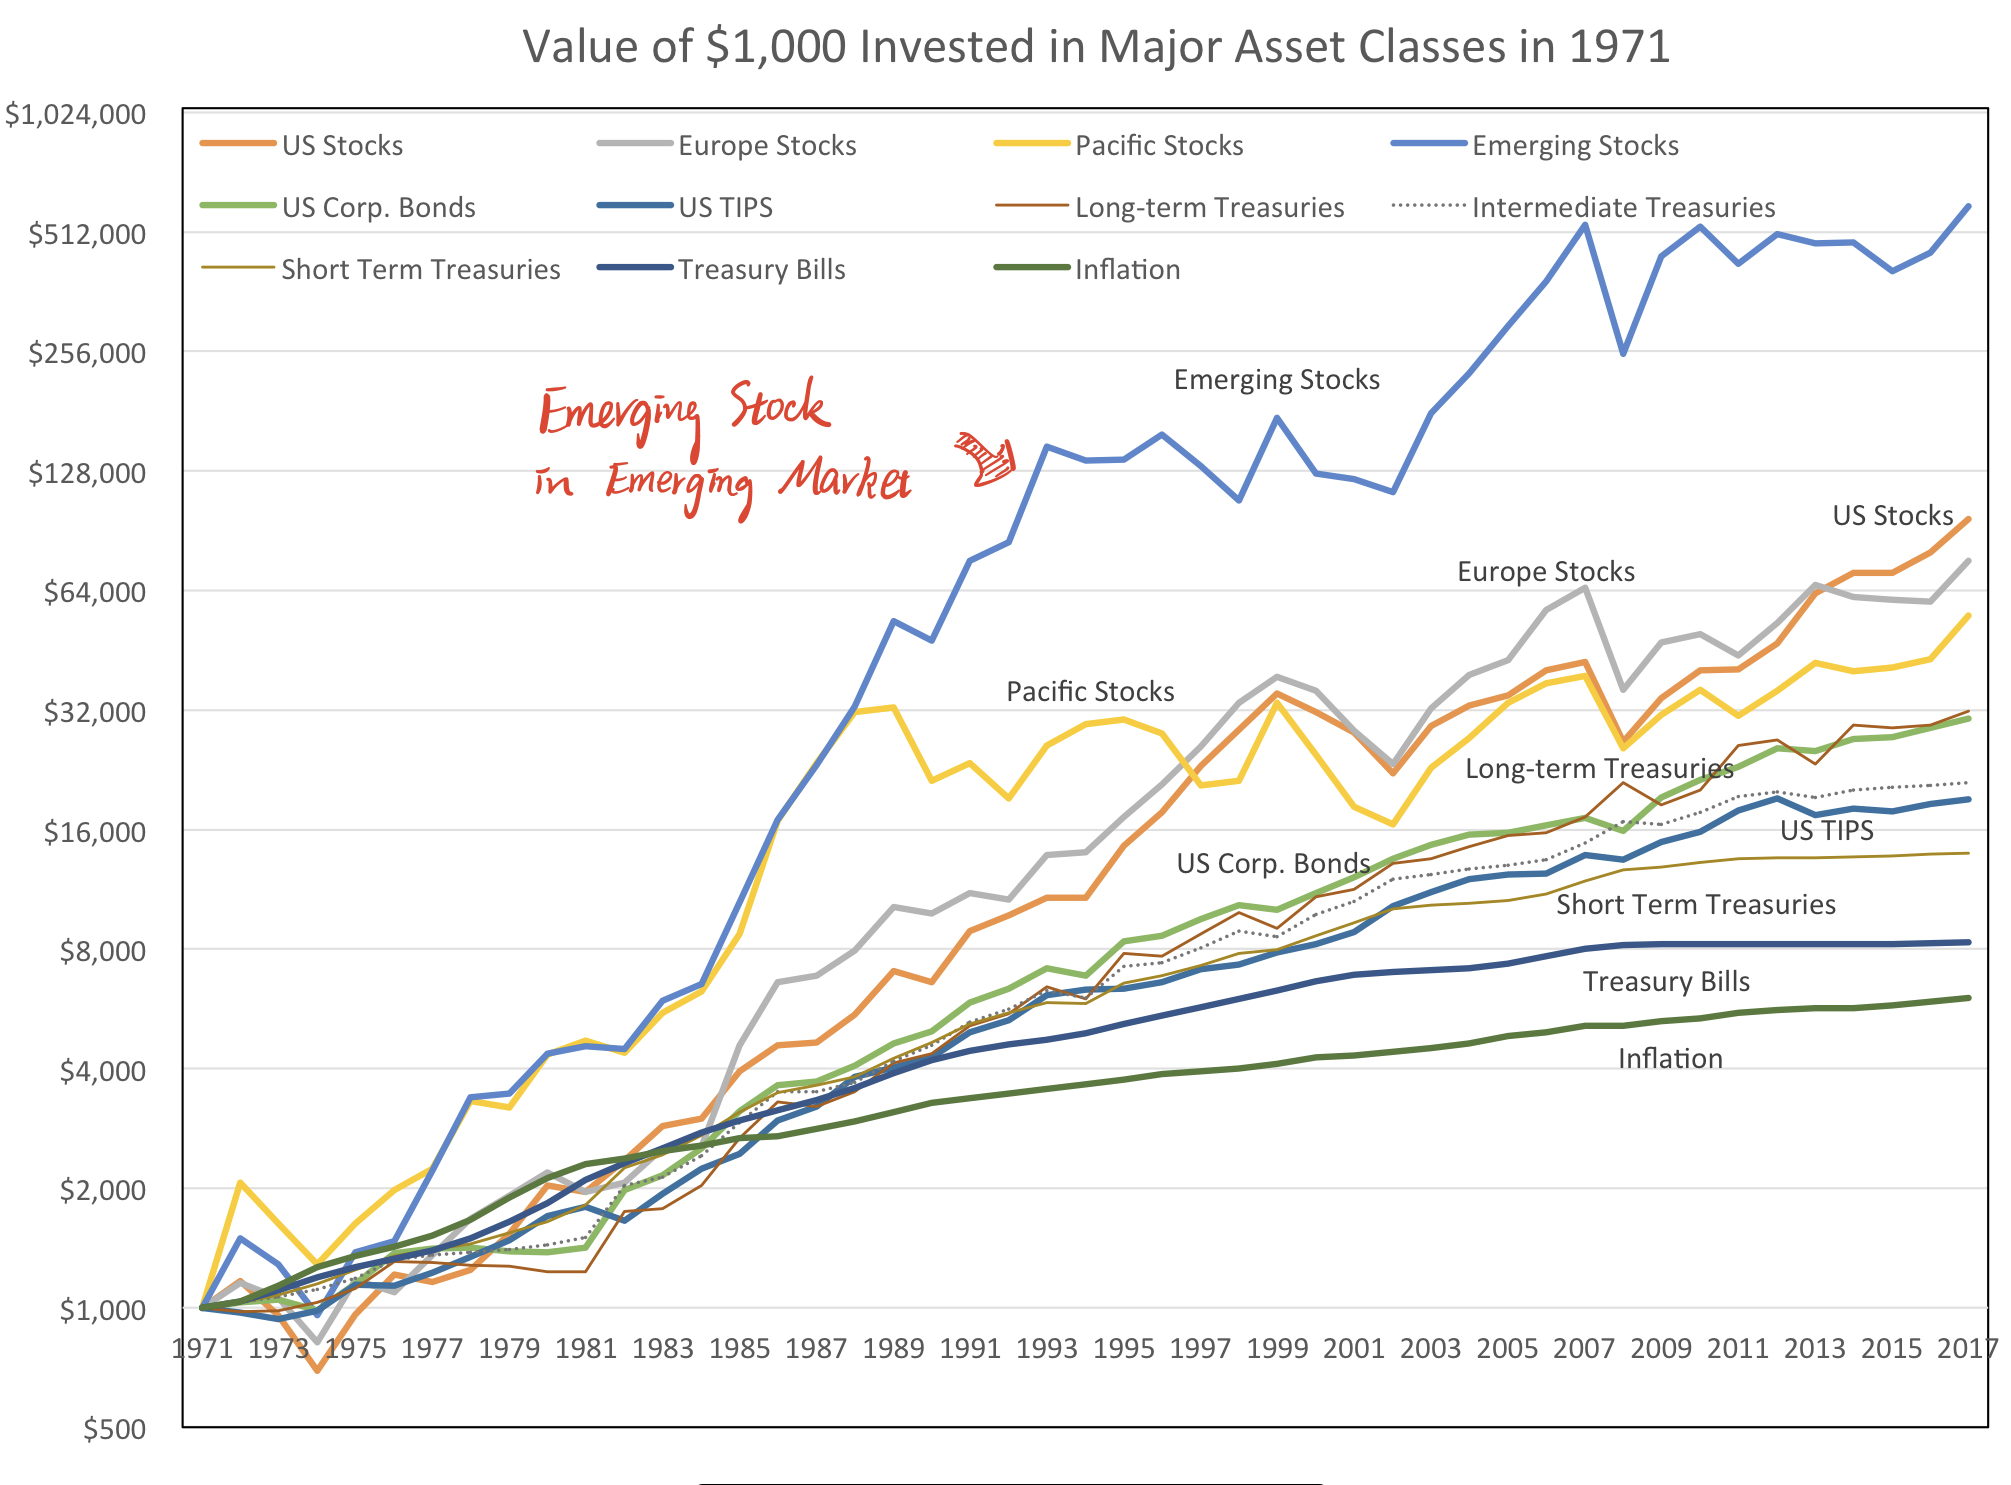
\includegraphics[width=0.6\textwidth]{asset_return_comparison_2}
%     \end{center}


\newpage
    \begin{center}
         \Large{\textbf{Overview}} \\
    \end{center}

    \subsection{\color{blue}A story of investing}
    
    Traditional paradigm focuses on \textbf{historical performance}, but they overlook \textbf{asset class allocation}. When thinking about return, we have to think in terms of {\color{red}three return sources:}
    \begin{itemize}
        \item Asset classes: stocks, bonds, alternative investments
        \item Strategy style: value, carry, momentum, etc
        \item Risk factors: growth, inflation, liquidity
    \end{itemize}

    With this concept in mind, investors can try to boost expected returns by:
    \begin{itemize}
         \item beta: taking risks that produce attractive rewards for all market participants (beta risks)
         \item alpha: by skillful active management (alpha) which may involve exploiting regularities and market inefficiencies.
    \end{itemize}

    But why the traditional way of using historical returns to forecast future returns didn't work:
    \begin{itemize}
        \item Bias: Any sample selection may be biased. For specific funds and strategies, the historical performance data that investors get to see are often upward biased. This bias is due to the voluntary nature of performance reporting and survivorship bias
        \item Relevence: In principle, longer historical windows reduce sample specificity and enable more accurate estimates of average returns. However, distant historical data may be irrelevant due to structural changes, apart from lower data quality.
        \item Cycle: Expected returns may vary over time in a cyclical fashion, which makes extrapolation of multi-year performance particularly dangerous.
    \end{itemize}

    In the old days, finance theories consist of \textbf{single-factor CAPM, efficient market, constant expected return}. However, nowadays we focus on expected return that is driven by the sources we listed above. A very important aspect of view change is that: \textbf{required asset return has little to do with asset's standalone volatility, but has more to do with when losses can be expected to occur}. Interestingly:
    \begin{itemize}
        \item Forward-looking indicators such as valuation ratios have a better track record in forecasting future asset class returns than rearview mirror measures.
        \item Long-run expected returns for any investment tend to be especially high following adverse events.
    \end{itemize}


            % $
            % \begin{cases}
            %     \text{}\\
            %     \text{}\\
            %     \text{}\\
            %     \text{}\\
            % \end{cases}
            % $

            % \includegraphics[width=0.8\textwidth]{}



% \newpage
%     \begin{center}
%          \Large{\textbf{Why investment with machine learning is so hard}} \\
%     \end{center}


    % \subsection{}
    % \begin{itemize}
    %     \item 
        % \item 
        % \item 
        % \item 
        % \item 
        % \item 
        % \item 
    % \end{itemize}


            % $
            % \begin{cases}
            %     \text{}\\
            %     \text{}\\
            %     \text{}\\
            %     \text{}\\
            % \end{cases}
            % $

            % \includegraphics[width=0.8\textwidth]{}

\end{document}